\subsection{OSN -- Основные методы обработки изображений: тональная коррекция, свёртка изображений, выделение краёв.}


\begin{itemize}
\item \textbf{Тональная коррекция} заключается в перераспределении света и тени между пикселями, то есть в регулировке яркости и контрастности изображения. 

\textit{ Как мы можем численно оценить, контрастным получилось изображение или нет?} При помощи оценки \textbf{гистограммы яркости} -- это график, где по горизонтальной оси отложены уровни яркости от 0 до 255, а по вертикальной оси число пикселей изображения.

Для определения яркости пикселя можно воспользоваться формулой Y=0.3*R+0.59*G+0.11*B, правда это больше для изображений в оттенках серого.


\item Часть диапазона, которая используется в изображении, называется его \textbf{тоновым диапазоном}. 

Крайняя слева точка гистограммы соответствует нулевой, а крайняя справа -- максимально возможной яркости. Чем шире тоновый диапазон, тем больше деталей может передать изображение и тем выше его качество. Условно тоновый диапазон делится на три части. Левая часть соответствует темным местам изображения, правая часть --- светлым местам, между ними находятся средние тона. В идеальном изображении присутствуют пиксели всех оттенков.
\item Что можно выявить:
    \item[--] Не полностью используется диапазон яркости;
    \item[--] Концентрация яркости вокруг определенных значений --- неравномерное заполнение диапазона яркости.
\end{itemize}



\textbf{Методы решения проблемы}
\begin{itemize}
\item \textbf{Линейная коррекция.} 
$f^{-1}(x) = y$; $x$ --- яркость пикселя на исходном изображении, $y$ --- яркость пикселя после коррекции. Компенсация узкого диапазона яркостей --- линейное растяжение гистограммы (histogram equalization):
$$y = \frac{(x-x_{min})\cdot(255-0)}{(x_{max} - x_{min})}$$

\item \textbf{Нелинейная коррекция}:\newline
\textit{Гамма-коррекция}. Изначальная цель -- коррекция для правильного отображения на мониторе, $y = c \cdot x^\gamma$;

\textit{Логарифмическая}. Цель -- сжатие динамического диапазона при визуализации данных, $y = c \cdot \log(1 + x)$. Тут $y$ --- яркость уже после коррекции.
\end{itemize}

\textbf{Свертка} --- это операция вычисления нового значения выбранного пикселя, учитывающая значения окружающих его пикселей.

Для вычисления значения используется матрица, называемая ядром свертки. Обычно ядро свертки является квадратной матрицей n * n, где n --- нечетное, однако ничто не мешает сделать матрицу прямоугольной.
Во время вычисления нового значения выбранного пикселя ядро свертки как бы <прикладывается> своим центром (именно тут важна нечетность размера матрицы) к данному пикселю. Окружающие пиксели так же накрываются ядром.
Далее высчитывается сумма, где слагаемыми являются произведения значений пикселей на значения ячейки ядра, накрывшей данный пиксель. Сумма делится на сумму всех элементов ядра свертки. Полученное значение как раз и является новым значением выбранного пикселя.
Если применить свертку к каждому пикселю изображения, то в результате получится некий эффект, зависящий от выбранного ядра свертки.

\textbf{Пространственная фильтрация. Линейные фильтры}

Под \textbf{фильтрацией} изображений понимают операцию, имеющую своим результатом изображение того же размера, полученное из исходного изображения по некоторым правилам.

Обычно интенсивность (цвет) каждого пикселя результирующего изображения обусловлена интенсивностями (цветами) пикселей, расположенных в некоторой его окрестности в исходном изображении. Это надо для борьбы с шумом на изображении.

\textbf{Алгоритм:} Заменим каждый пиксель взвешенным средним по окрестности. Веса обозначаются как ядро фильтра. Веса для усреднения задаются в виде квадратной матрицы k * k. \newline
Пусть $f$ --- изображение, $g$ --- ядро. Свертка f по g тогда обозначается как $f*g$: $(f * g)[m,n] = \sum f(m-k,n-l)*g(k,l)$, где $k,l$ пробегают число строк/столбцов матрицы $g$ --- так и получаем усреднение.

\textbf{Основные свойства линейных фильтров:}
\begin{itemize}
    \item Линейность: 
    
    $filter(f_1 + f_2) = filter(f_1) + filter(f_2)$
    
    $filter(a * f_1) = a * filter(f_1)$
    
    \item Инвариантность к сдвигу --- не зависит от сдвига пиксела: 
    
    $filter(shift(f)) = shift(filter(f))$
    
    \textbf{Теорема.} Любой линейный оператор, инвариантный к сдвигу, может быть записан в виде свертки.
    
\end{itemize}

\textbf{Примеры фильтров:}
\begin{itemize}
    \item box-фильтр;  
    \item Фильтр Гаусса;
    \item Медианный --- меняет значение на медиану по фильтру (это нелинейный фильтр --- вдруг спросят);
    \item unsharp (повышение резкости)
\end{itemize}

Линейная фильтрация (свёртка) изображения позволяет решать целый ряд
задач --- шумоподавление, повышение резкости, оценка градиента. \newline

\textbf{Выделение краев}

\textbf{Задача:} выделить резкие изменения (разрывы) изображения. Край --- это точка резкого изменения значений функции интенсивности изображения.

\begin{itemize}
\item Градиент изображения: $\nabla f = \left[ \frac{\partial f}{\partial x}, \frac{\partial f}{\partial y} \right]$. Градиент направлен в сторону наибольшего изменения интенсивности.
\item Сила края задается величиной (нормой) градиента:
$$  \| \nabla f  \| = \sqrt{\Big(\frac{\partial f}{\partial x}\Big)^2 + \Big(\frac{\partial f}{\partial y}\Big)^2}$$
\item Разностная производная (для функции 2-х переменных):\newline
$\frac{\partial f}{\partial x} \approx \frac{f(x_{n+1},y)-f(x_n,y)}{\Delta x} $ -- это свёртка. 

\end{itemize}

Задачу выделения краёв изображения в простом случае можно решить как поиск локальных максимумов градиента яркости. \newline
После получения силы края во всех точках можно по-разному определять края -- отсекать по пороговому значению, выделять локальные максимумы для утоньшения краёв и повышения точности, отсекать по гистерезису (для начала построения кривой границы порог большой, для продолжения порог ниже).

\textbf{Фильтр Собеля} (Sobel filter)

Используются свертки 3*3, с помощью которых аппрокимируются производные -- горизонтальная и вертикальная. Пусть $F$ -- исходное изображение, $G_x$ and $G_y$ -- изображения которые в каждой точке содержат приближение горизонтальной и вертикальной производных.

$$
G_x = 
\begin{bmatrix}
+1 & 0 & -1 \\
+2 & 0 & -2 \\
+1 & 0 & -1 \\
\end{bmatrix}
* F, ~ 
G_y = 
\begin{bmatrix}
+1 & +2 & +1 \\
0  & 0  & 0  \\
-1 & -2 & -1 \\
\end{bmatrix}
* F
$$

где * означает операцию свертки.

x здесь <<увеличивается>> вправо, y - вниз. В каждой точке можно объединить их и получить модуль градиента.

$$G = \sqrt{G_x^2 + G_y^2}$$

Пример из Википедии: До и после фильтра Собеля

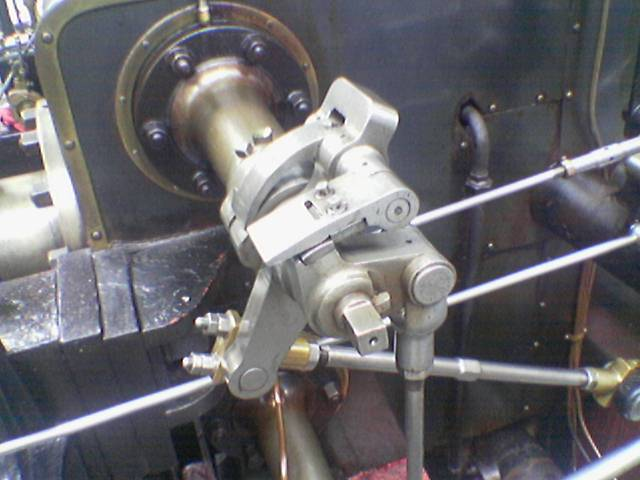
\includegraphics[scale=0.2]{pics/osn23_before.png}
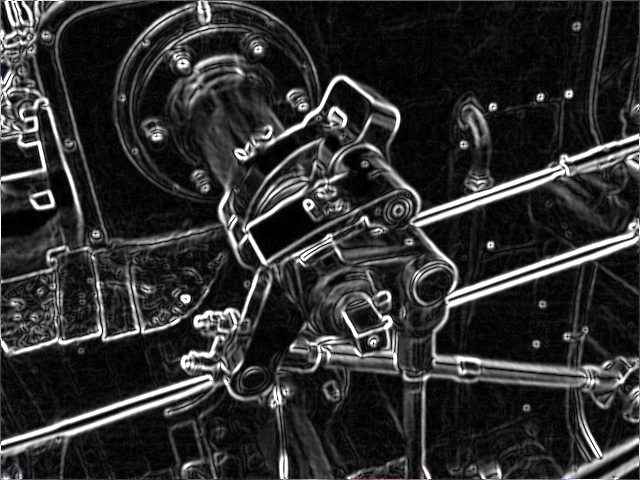
\includegraphics[scale=0.2]{pics/osn23_after.png}

% -------- source --------
\bigbreak
[\cite[page 69-96]{replace_me}]